\documentclass[12pt]{article}
\usepackage[margin=1in]{geometry} 
\usepackage{amsmath,amsthm,amssymb,amsfonts,mathtools}
\usepackage{fancyhdr}
\usepackage{graphicx}
\graphicspath{ {./figures/} }

\newenvironment{problem}[2][]{
    \begin{trivlist}
        \item[
            {\bfseries #1}
            {\bfseries #2}
        ]
}{\end{trivlist}}

\newcommand{\chaptertitle}{Chapter 2 Motion Along A Straight Line}
\newcommand{\sectiontitle}{\textsc{2.3 Average and Instantaneous Acceleration}}
\newcommand{\name}{\textsc{Eric Nguyen}}

\pagestyle{fancy}
\chead{\sectiontitle \hfill \textsc{\today} \hfill \name}
\cfoot{\thepage}
\setlength{\headheight}{15pt}

\newcommand{\solution}{\medskip\noindent\textbf{Solution:}}
\newcommand{\Part}[1]{\shortintertext{(#1)}}
\newcommand{\PPart}[1]{\shortintertext{\qquad(#1)}}
\newcommand{\where}{, \, \text{ where }}
\newcommand{\magnitude}[1]{\lVert #1 \rVert}
\newcommand{\Vector}[2]{\langle #1, #2 \rangle}
\newcommand{\UVector}[2]{\left(#1\right)\ihat + \left(#2\right)\jhat}
\newcommand{\ihat}{\hat{\imath}}
\newcommand{\jhat}{\hat{\jmath}}

% UNITS
\newcommand{\unit}[1]{\, \text{#1}}

\newcommand{\cm}{\unit{cm}}
\newcommand{\m}{\unit{m}}
\newcommand{\km}{\unit{km}}
\newcommand{\ft}{\unit{ft}}
\newcommand{\inch}{\unit{in.}}
\newcommand{\mi}{\unit{mi}}
\newcommand{\gcm}{\unit{g/cm}}
\newcommand{\mum}{\, \mu \text{m}}
\newcommand{\mm}{\unit{mm}}

\newcommand{\Liter}{\unit{L}}
\newcommand{\gallon}{\unit{gallon}}
\newcommand{\kg}{\unit{kg}}
\newcommand{\g}{\unit{g}}
\newcommand{\lb}{\unit{lb}}

\newcommand{\mph}{\unit{mi/h}}
\newcommand{\kmh}{\unit{km/h}}
\newcommand{\cms}{\unit{cm/s}}
\newcommand{\mps}{\unit{m/s}}
\newcommand{\mpg}{\unit{mpg}}
\newcommand{\kmL}{\unit{km/L}}

\newcommand{\y}{\unit{y}}
\newcommand{\mo}{\unit{mo}}
\newcommand{\ns}{\unit{ns}}
\newcommand{\s}{\unit{s}}
\newcommand{\gs}{\unit{gs}}
\newcommand{\days}{\unit{days}}
\newcommand{\Day}{\unit{day}}
\newcommand{\hours}{\unit{hrs}}
\newcommand{\hour}{\unit{hr}}
\newcommand{\Hour}{\unit{h}}
\newcommand{\minutes}{\unit{mins}}
\newcommand{\minute}{\unit{min}}

\newcommand{\ftpns}{\unit{ft/ns}}
\newcommand{\nspft}{\unit{ns/ft}}

\begin{document}

\begin{problem}{2.13}
    \textbf{The Fastest (and Most Expensive) Car!} The table shows test data for the Bugatti Veyron Super Sport, the fastest street car made.
    The car is moving in a straight line (the $x$-axis).

    \bigskip

    \begin{tabular}{l*{5}{c}r}
        \textbf{Time (s)} & 0 & 2.1 & 20.0 & 53 \\
        \textbf{Speed (mi/h)} & 0 & 60 & 200 & 253
    \end{tabular}

    \bigskip

    \noindent (a) Sketch a $v_x$-$t$ graph of this car's velocity (in mi/h) as a function of time. Is its acceleration constant?
    (b) Calculate the car's average acceleration in (m/s$^2$) between
    (i) 0 and 2.1 s;
    (ii) 2.1 s and 20.0;
    (iii) 20.0 s and 53 s.
    Are these results consistent with your graph in part (a)?
    (Before you decide to buy this car, it might be helpful to know that only 300 will be built, it runs out of gas in 12 minutes at top speed, and it costs more than \$1.5 million!)

    \solution
    \begin{align}
        \Part{a}
        &% GNUPLOT: LaTeX picture
\setlength{\unitlength}{0.240900pt}
\ifx\plotpoint\undefined\newsavebox{\plotpoint}\fi
\sbox{\plotpoint}{\rule[-0.200pt]{0.400pt}{0.400pt}}%
\begin{picture}(937,562)(0,0)
\sbox{\plotpoint}{\rule[-0.200pt]{0.400pt}{0.400pt}}%
\put(151.0,131.0){\rule[-0.200pt]{4.818pt}{0.400pt}}
\put(131,131){\makebox(0,0)[r]{$0$}}
\put(856.0,131.0){\rule[-0.200pt]{4.818pt}{0.400pt}}
\put(151.0,196.0){\rule[-0.200pt]{4.818pt}{0.400pt}}
\put(131,196){\makebox(0,0)[r]{$50$}}
\put(856.0,196.0){\rule[-0.200pt]{4.818pt}{0.400pt}}
\put(151.0,261.0){\rule[-0.200pt]{4.818pt}{0.400pt}}
\put(131,261){\makebox(0,0)[r]{$100$}}
\put(856.0,261.0){\rule[-0.200pt]{4.818pt}{0.400pt}}
\put(151.0,326.0){\rule[-0.200pt]{4.818pt}{0.400pt}}
\put(131,326){\makebox(0,0)[r]{$150$}}
\put(856.0,326.0){\rule[-0.200pt]{4.818pt}{0.400pt}}
\put(151.0,391.0){\rule[-0.200pt]{4.818pt}{0.400pt}}
\put(131,391){\makebox(0,0)[r]{$200$}}
\put(856.0,391.0){\rule[-0.200pt]{4.818pt}{0.400pt}}
\put(151.0,456.0){\rule[-0.200pt]{4.818pt}{0.400pt}}
\put(131,456){\makebox(0,0)[r]{$250$}}
\put(856.0,456.0){\rule[-0.200pt]{4.818pt}{0.400pt}}
\put(151.0,521.0){\rule[-0.200pt]{4.818pt}{0.400pt}}
\put(131,521){\makebox(0,0)[r]{$300$}}
\put(856.0,521.0){\rule[-0.200pt]{4.818pt}{0.400pt}}
\put(151.0,131.0){\rule[-0.200pt]{0.400pt}{4.818pt}}
\put(151,90){\makebox(0,0){$0$}}
\put(151.0,501.0){\rule[-0.200pt]{0.400pt}{4.818pt}}
\put(272.0,131.0){\rule[-0.200pt]{0.400pt}{4.818pt}}
\put(272,90){\makebox(0,0){$10$}}
\put(272.0,501.0){\rule[-0.200pt]{0.400pt}{4.818pt}}
\put(393.0,131.0){\rule[-0.200pt]{0.400pt}{4.818pt}}
\put(393,90){\makebox(0,0){$20$}}
\put(393.0,501.0){\rule[-0.200pt]{0.400pt}{4.818pt}}
\put(514.0,131.0){\rule[-0.200pt]{0.400pt}{4.818pt}}
\put(514,90){\makebox(0,0){$30$}}
\put(514.0,501.0){\rule[-0.200pt]{0.400pt}{4.818pt}}
\put(634.0,131.0){\rule[-0.200pt]{0.400pt}{4.818pt}}
\put(634,90){\makebox(0,0){$40$}}
\put(634.0,501.0){\rule[-0.200pt]{0.400pt}{4.818pt}}
\put(755.0,131.0){\rule[-0.200pt]{0.400pt}{4.818pt}}
\put(755,90){\makebox(0,0){$50$}}
\put(755.0,501.0){\rule[-0.200pt]{0.400pt}{4.818pt}}
\put(876.0,131.0){\rule[-0.200pt]{0.400pt}{4.818pt}}
\put(876,90){\makebox(0,0){$60$}}
\put(876.0,501.0){\rule[-0.200pt]{0.400pt}{4.818pt}}
\put(151.0,131.0){\rule[-0.200pt]{0.400pt}{93.951pt}}
\put(151.0,131.0){\rule[-0.200pt]{174.652pt}{0.400pt}}
\put(876.0,131.0){\rule[-0.200pt]{0.400pt}{93.951pt}}
\put(151.0,521.0){\rule[-0.200pt]{174.652pt}{0.400pt}}
    \put(0,326){\rotatebox[origin=c]{90}{Speed (mi/h)}}
\put(513,29){\makebox(0,0){Time (s)}}
\put(151,131){\usebox{\plotpoint}}
\multiput(151.58,131.00)(0.497,1.574){47}{\rule{0.120pt}{1.348pt}}
\multiput(150.17,131.00)(25.000,75.202){2}{\rule{0.400pt}{0.674pt}}
\multiput(176.00,209.58)(0.596,0.500){361}{\rule{0.577pt}{0.120pt}}
\multiput(176.00,208.17)(215.803,182.000){2}{\rule{0.288pt}{0.400pt}}
\multiput(393.00,391.58)(2.896,0.499){135}{\rule{2.407pt}{0.120pt}}
\multiput(393.00,390.17)(393.004,69.000){2}{\rule{1.204pt}{0.400pt}}
\put(151,131){\makebox(0,0){$\bullet$}}
\put(176,209){\makebox(0,0){$\bullet$}}
\put(393,391){\makebox(0,0){$\bullet$}}
\put(791,460){\makebox(0,0){$\bullet$}}
\put(151.0,131.0){\rule[-0.200pt]{0.400pt}{93.951pt}}
\put(151.0,131.0){\rule[-0.200pt]{174.652pt}{0.400pt}}
\put(876.0,131.0){\rule[-0.200pt]{0.400pt}{93.951pt}}
\put(151.0,521.0){\rule[-0.200pt]{174.652pt}{0.400pt}}
\end{picture}
 \\
        &\text{The acceleration of the car is not constant.}
        \Part{b}
        a_{\text{av-}x} &= \frac{\Delta v_x}{\Delta t} = \frac{v_{2x} - v_{1x}}{t_2 - t_1} \\
        \PPart{i}
        a_{\text{av-}x} &= \frac{60 \mph - 0 \mph}{2.1 \s - 0 \s} \\
        &= \frac{60 \mi}{2.1 \s \cdot \text{h}} \left(\frac{1 \Hour}{60 \minutes}\right) \left(\frac{1 \minute}{60 \s}\right) \left(\frac{1.609 \km}{1 \mi}\right) \left(\frac{1000 \m}{1 \km}\right) \\
        &= \frac{96,540 \m}{7,560 \s^2} \approx 12.8 \mps^2
        \PPart{ii}
        a_{\text{av-}x} &= \frac{200 \mph - 60 \mph}{20.0 \s - 2.1 \s} \\
        &= \frac{140 \mi}{17.9 \s \cdot \Hour} \left(\frac{1 \Hour}{60 \minutes}\right) \left(\frac{1 \minute}{60 \s}\right) \left(\frac{1.609 \km}{1 \mi}\right) \left(\frac{1000 \m}{1 \km}\right) \\
        &= \frac{225,260 \m}{64,440 \s^2} \approx 3.50 \mps^2
        \PPart{iii}
        a_{\text{av-}x} &= \frac{253 \mph - 200 \mph}{53 \s - 20.0 \s} \\
        &= \frac{53 \mi}{33 \s \cdot \Hour} \left(\frac{1 \Hour}{60 \minutes}\right) \left(\frac{1 \minute}{60 \s}\right) \left(\frac{1.609 \km}{1 \mi}\right) \left(\frac{1000 \m}{1 \km}\right) \\
        &= \frac{85,277 \m}{118,800 \s^2} \approx 0.718 \mps^2
    \end{align}
\end{problem}

\begin{problem}{2.15}
    A turtle crawls along a straight line, which we will call the $x$-axis with the positive direction to the right.
    The equation for the turtle's position as a function of time is $x(t) = 50.0 \text{ cm } + (2.00 $ cm/s$)t - (0.0625$ cm/s$^2)t^2$.
    (a) Find the turtle's initial velocity, initial position, and inital acceleration.
    (b) At what time $t$ is the velocity of the turtle zero?
    (c) How long after starting does it take the turtle to return to its
    starting point?
    (d) At what time $t$ is the turtle a distance of 10.0 cm from its starting point?
    What is the velocity (magnitude and direction) of the turtle at each of those times?
    (e) Sketch graphs of $x$ versus $t$, $v_x$ versus $t$, and $a_x$ versus $t$, for the time interval $t = 0$ to $t = 40$ s.

    \solution
    \begin{align}
        x(t) &= 50.0 \cm + \left(2.00 \cms\right) t - \left(0.0625 \cms^2\right) t^2 \\
        v(t) &= x'(t) = \left(2.00 \cms\right) - 2 \left(0.0625 \cms^2\right) t \\
        &\phantom{=. x'(t)} = \left(2.00 \cms\right) - \left(0.125 \cms^2\right) t \\
        a(t) &= v'(t) = -\left(0.125 \cms^2\right)
        \Part{a}
        x_0 &= x(0 \s) = 50.0 \cm \\
        v_0 &= v(0 \s) = \left(2.00 \cms\right) - \left(0.125 \cms^2\right) \left(0 \s\right) = 2.00 \cms \\
        a_0 &= a(0 \s) = -0.125 \cms^2
        \Part{b}
        0 &= \left(2.00 \cms\right) - \left(0.125 \cms^2\right) t \\
        - \left(2.00 \cms\right) &= - \left(0.125 \cms^2\right) t \\
        t &= \frac{- \left(2.00 \cms\right)}{- \left(0.125 \cms^2\right)} = 16.0 \s \\
        \Part{c}
        50.0 \cm &= 50.0 \cm + \left(2.0 \cms\right) t - \left(0.0625 \cms^2\right) t^2 \\
        0 \cm &= t \left[\left(2.00 \cms\right) - \left(0.0625 \cms^2\right) t\right] \\
        - 2.00 \cms &= - \left(0.0625 \cms^2\right) t \\
        t &= \frac{- 2.00 \cms}{- 0.0625 \cms^2} = 32.0 \s \\
        \Part{d}
        60.0 \cm &= 50.0 \cm + \left(2.00 \cms\right) t - \left(0.0625 \cms^2\right) t^2 \\
        0 &= \left(0.0625 \cms^2\right) t^2 - \left(2.00 \cms\right) t + 10.0 \cm \\
        t &= \frac{-b \pm \sqrt{b^2 - 4ac}}{2a} \\
        &= \frac{\left(2.00 \cms\right) \pm \sqrt{\left(2.00 \cms\right)^2 - 4 \left(0.0625 \cms^2\right) \left(10.0 \cm\right)}}{2 \left(0.0625 \cms^2\right)} \\
        &\approx 6.20 \s \text{ and } 25.8 \s \\
        40.0 \cm &= 50.0 \cm + \left(2.00 \cms\right) t - \left(0.0625 \cms^2\right) t^2 \\
        0 &= \left(0.0625 \cms^2\right) t^2 - \left(2.00 \cms\right) t - 10.0 \cm \\
        t &= \frac{\left(2.00 \cms\right) \pm \sqrt{\left(2.00 \cms\right)^2 - 4 \left(0.0625 \cms^2\right) \left(-10.0 \cm\right)}}{2 \left(0.0625 \cms^2\right)} \\
        &\approx 36.4 \s \\
        v(6.20 \s) &= \left(2.00 \cms\right) - \left(0.125 \cms^2\right) (6.20 \s) \approx 1.23 \mps \\
        v(25.8 \s) &= \left(2.00 \cms\right) - \left(0.125 \cms^2\right) (25.8 \s) \approx -1.23 \mps \\
        v(36.4 \s) &= \left(2.00 \cms\right) - \left(0.125 \cms^2\right) (36.4 \s) \approx -2.55 \mps
        \Part{e}
        &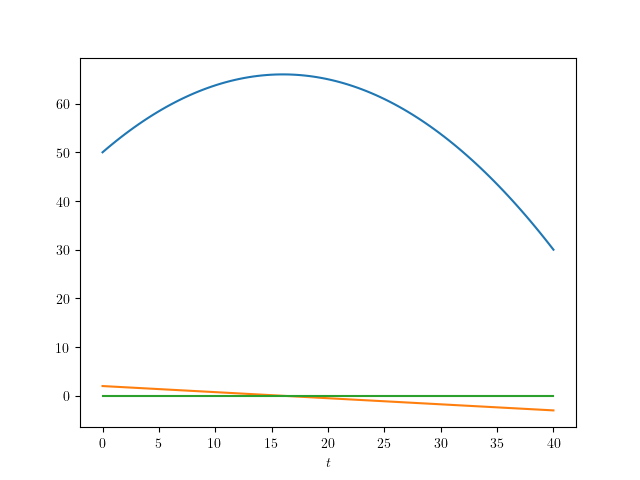
\includegraphics[scale=0.55]{2_15.png}
    \end{align}
\end{problem}

\clearpage

\begin{problem}{2.17}
    A car's velocity as a function of time is given by $v_x(t) = \alpha + \beta t^2$, where $\alpha = 3.00$ m/s and $\beta = 0.100$ m/s$^3$.
    (a) Calculate the average acceleration for the time interval $t = 0$ to $t = 5.00$ s.
    (b) Calculate the instantaneous acceleration for $t = 0$ and $t = 5.00$ s.
    (c) Draw $v_x$-$t$ and $a_x$-$t$ graphs for the car's motion between $t = 0$ and $t = 5.00$ s.

    \solution
    \begin{align}
        \Part{a}
        v_{2x} &= v_x(5.00 \s) = \left(3.00 \mps\right) + \left(0.100 \mps^3\right) \left(5.00 \s\right)^2 = 5.50 \mps \\
        v_{1x} &= v_x(0 \s) = \left(3.00 \mps\right) + \left(0.100 \mps^3\right) \left(0 \s\right)^2 = 3.00 \mps \\
        a_{\text{av-}x} &= \frac{\Delta v_x}{\Delta t} = \frac{v_{2x} - v_{1x}}{t_2 - t_1} = \frac{5.5 \mps - 3.0 \mps}{5.00 \s - 0 \s} = 0.500 \mps^2
        \Part{b}
        a_x &= \underset{\Delta t \to 0}{\lim} \frac{\Delta v_x}{\Delta t} = \frac{dv_x}{dt} = \frac{d}{dt} \left[\left(3.00 \mps\right) + \left(0.100 \mps^3\right) t^2\right] \\
        &= \left(0.200 \mps^3\right) t \\
        a_x(0 \s) &= \left(0.200 \mps^3\right) \left(0 \s\right) = 0 \mps^2 \\
        a_x(5.00 \s) &= \left(0.200 \mps^3\right) \left(5.00 \s\right) = 1.00 \mps^2
        \Part{c}
        &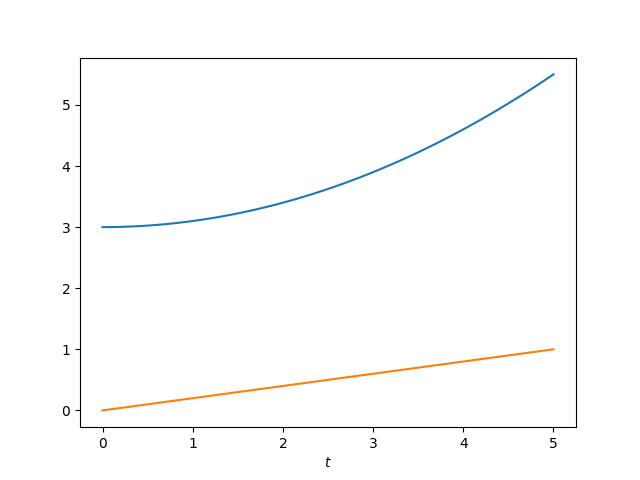
\includegraphics[scale=0.55]{2_17.png}
    \end{align}
\end{problem}

\end{document}

